%-----------------------------------------------------------------
% BAB IV HASIL DAN PEMBAHASAN
%
% Struktur sesuai panduan penulisan tesis:
%   4.1 Hasil dan Pembahasan 1
%   4.2 Hasil dan Pembahasan 2
%   4.3 Hasil dan Pembahasan 3
%-----------------------------------------------------------------
\chapter{HASIL DAN PEMBAHASAN}

% Struktur bab mengikuti panduan. Setiap subbab sebaiknya diberi judul
% yang menjelaskan topik pembahasannya, bukan sekadar nomor.
% Ganti isi tiap subbab dengan hasil penelitian Anda.

\section{Hasil dan Pembahasan 1}

Sajikan hasil penelitian dan pembahasan pada subbab ini. Rujukan dari
`daftar-pustaka.bib` memakai perintah \cite{buku2020}.

% \subsection{[Judul Subbab]}

\section{Hasil dan Pembahasan 2}

Sajikan hasil penelitian dan pembahasan pada subbab ini.

% \subsection{[Judul Subbab]}

\section{Hasil dan Pembahasan 3}

Sajikan hasil penelitian dan pembahasan pada subbab ini.

%-----------------------------------------------------------------
% Tabel dan gambar contoh. Hapus bila tidak dipakai pada naskah Anda.
%-----------------------------------------------------------------
% \begin{table}[ht]
% \centering
% \caption{[Judul Tabel]}
% \begin{tabular}{cc}
% \toprule
% No & Keterangan \\
% \midrule
% 1 & \\
% \bottomrule
% \end{tabular}
% \label{tab:contoh}
% \end{table}

% \begin{figure}[ht]
% \centering
%     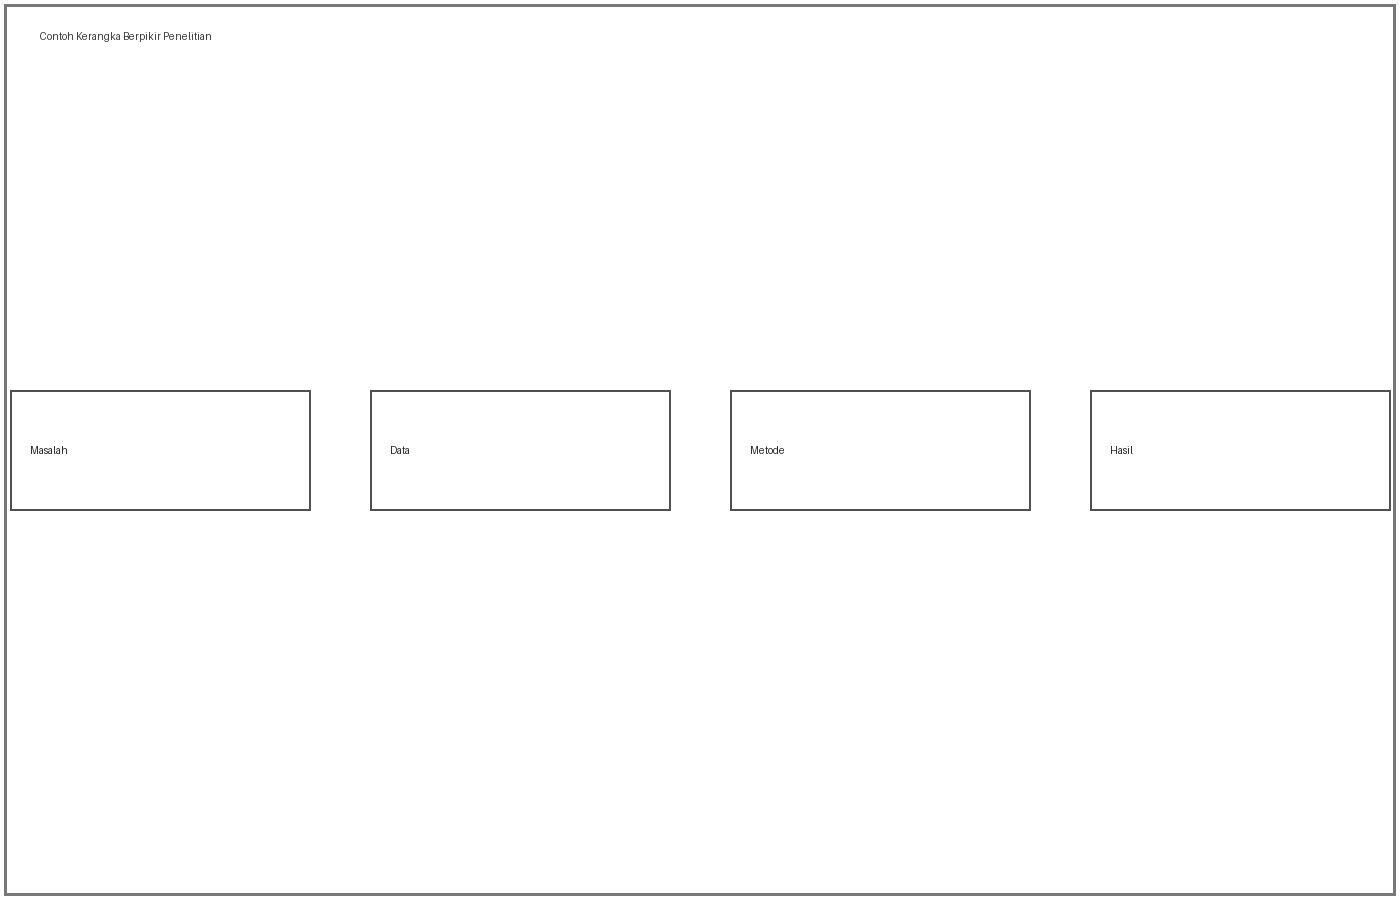
\includegraphics[width=0.8\textwidth]{image/contoh-kerangka-berpikir.png}
%     \caption{[Judul Gambar]}
%     \label{fig:contoh}
% \end{figure}